\documentclass[11pt, oneside]{article}   	% use "amsart" instead of "article" for AMSLaTeX format
\usepackage{geometry}                		% See geometry.pdf to learn the layout options. There are lots.
\geometry{letterpaper}                   		% ... or a4paper or a5paper or ... 
%\geometry{landscape}                		% Activate for rotated page geometry
%\usepackage[parfill]{parskip}    		% Activate to begin paragraphs with an empty line rather than an indent
\usepackage{graphicx}				% Use pdf, png, jpg, or eps§ with pdflatex; use eps in DVI mode
								% TeX will automatically convert eps --> pdf in pdflatex		
\usepackage{amssymb}
\usepackage{amsthm}
 \usepackage{hyperref}
  \usepackage{float}
%SetFonts

%SetFonts


\title{A note on ensemble learning}
\author{Yapi Donatien Achou}
%\date{}							% Activate to display a given date or no date

\begin{document}
\maketitle
\section{Introduction}
Ensemble learning models are obtained by combining simple base models in order to obtain a much more performant model. 
\section{Bagging methods}
\section{Boosting methods}
\subsection{AdaBoost}
The idea of AdaBoost is to train a weak classifier on weighted versions of the original training dataset and make the final prediction based on weighted majority vote.
Let $G_{m}, m = 1,2,\dots$,M be a weak classifier defines such that it performance is slightly worse or better than random guess.
Let $D_{1}$ be the training sample and $D_{2}, D_{3}$, $\dots$, $D_{M} $ be weighted samples obtained from the original training data set. By sequentially applying $G_{1}, G_{2}, \dots, G_{M}$ to the data set, $D_{2}, D_{3}$, $\dots$, $D_{M} $, a much better model $G$ is obtained by combining $G_{1}, G_{2}, \dots, G_{M}$ through a weighted majority vote such that 

\begin{equation}
G(x)= sign\left(  \sum_{m=1}^{M} \alpha_{m}G_{m}(x) \right)
\end{equation}

where the weights $\alpha_{m}, m = 1,2,\dots, M$ are obtained from the boosting algorithm and weight the contribution of each $G_{m}$ \cite{trevor}. At iteration $m$, misclassified training examples by classifier $G_{m-1}$ have their weight increased, while correctly classified training example have their weight decrease. This insures that training examples that are difficult to classify receive more attentions, by making sure that the next classifier concentrates on the training examples that are missed by previous one \cite{trevor}. This procedure improves the performance of the weak classifier at each iteration.
\begin{figure}[H] %  figure placement: here, top, bottom, or page
   \centering
   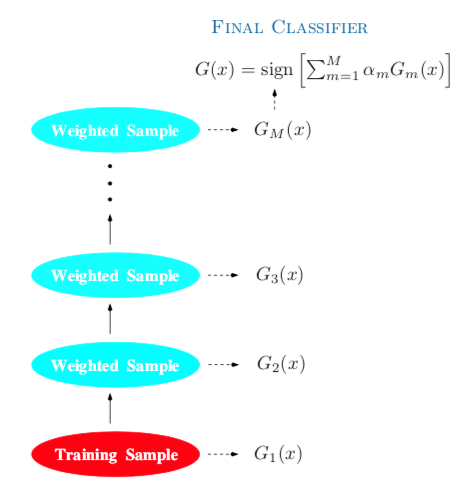
\includegraphics[width=4in]{adaboost.png} 
   \caption{Schematic description of AdaBoost algorithm. Picture taken from \cite{trevor}}
   \label{fig:adaboost}
\end{figure}
Figure \ref{fig:adaboost} shows the description of AdaBoost







%%%%%%%%%%%%%%%%%%%%%%%%%%%%%%%%%%%%%%%%%%%%%%%%%%%%%%%%%%%%%%%%%%
%%%%%%%%%%%%%%%%%%%%%%%%%%%%%%%%%%%%%%%%%%%%%%%%%%%%%%%%%%%%%%%%%%
%%%%%%%%%%%%%%%%%%%%%%%%%%%%%%%%%%%%%%%%%%%%%%%%%%%%%%%%%%%%%%%%%%
\medskip
\begin{thebibliography}{9}
\bibitem{chollet} 
Chollet, Fran\c{c}ois and others
\textit{Keras, \url{https://keras.io}}. 
2015


\bibitem{goodfellow} 
Ian Goodfellow and Yoshua Bengio and Aaron Courville
\textit{Deep Learning}. 
\url{http://www.deeplearningbook.org}, 2016

\bibitem{trevor} 
Trevor Hastie, Robert Tibshirani, Jerome Friedman
\textit{The Elements of Statistical Learning}. 
Springer Series in Statistics. 2008






 
\end{thebibliography}

\end{document}  